% Created 2015-08-23 Sun 14:45
\documentclass[presentation]{beamer}
\usepackage[utf8]{inputenc}
\usepackage[T1]{fontenc}
\usepackage{fixltx2e}
\usepackage{graphicx}
\usepackage{longtable}
\usepackage{float}
\usepackage{wrapfig}
\usepackage{rotating}
\usepackage[normalem]{ulem}
\usepackage{amsmath}
\usepackage{textcomp}
\usepackage{marvosym}
\usepackage{wasysym}
\usepackage{amssymb}
\usepackage{hyperref}
\tolerance=1000
\usepackage{tabu}
\usepackage{minted}
\hypersetup{pdfauthor="Vasilij Schneidermann", pdftitle="Emacs as my Canvas", colorlinks, linkcolor=black, urlcolor=blue}
\usetheme{Rochester}
\usecolortheme[RGB={87,83,170}]{structure}
\author{Vasilij Schneidermann}
\date{August 2015}
\title{Emacs as my Canvas}
\hypersetup{
  pdfkeywords={},
  pdfsubject={},
  pdfcreator={Emacs 24.5.1 (Org mode 8.2.10)}}
\begin{document}

\maketitle
\begin{frame}{Outline}
\tableofcontents
\end{frame}

\AtBeginSection{\frame{\sectionpage}}

\section{Introduction}
\label{sec-1}

\begin{frame}[label=sec-1-1]{Who?}
\begin{itemize}
\item Vasilij Schneidermann, 23
\item Information systems student
\item Working at bevuta IT, Cologne
\item \texttt{v.schneidermann@gmail.com}
\item \url{https://github.com/wasamasa}
\item \url{http://emacshorrors.com/}
\end{itemize}
\end{frame}

\begin{frame}[label=sec-1-2]{What?}
\begin{itemize}
\item Emacs is an extensible, \href{http://steve-yegge.blogspot.de/2007/01/pinocchio-problem.html}{QWAN} platform for all things text
\item Very fun to hack on
\item Yet very little graphical demos
\item Let's change that!
\end{itemize}
\end{frame}

\begin{frame}[label=sec-1-3]{Why?}
\begin{figure}[htb]
\centering
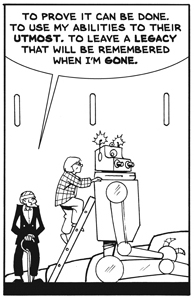
\includegraphics[height=4cm]{./images/why.jpg}
\caption{The Mad Scientist}
\end{figure}

\url{http://lastmechanicalmonster.blogspot.com/2014/08/page-91.html}
\end{frame}

\section{Basics}
\label{sec-2}

\begin{frame}[label=sec-2-1]{Emacs}
\begin{itemize}
\item A text editor from 1985
\item Ported to all kinds of common and lesser common platforms
\item Mostly implemented in Emacs Lisp
\item Extensible at runtime
\item Many interesting features
\end{itemize}
\end{frame}

\begin{frame}[label=sec-2-2]{Buffers}
\begin{itemize}
\item Basic data structure
\item Basically two strings and a gap
\item Can represent both files and text in memory
\item Used heavily for text processing
\end{itemize}
\end{frame}

\begin{frame}[fragile,label=sec-2-3]{Text Properties}
 \begin{itemize}
\item Supported for both strings and buffers
\item Property-value pairs attached to ranges of characters
\item Some of the properties are special, like \texttt{face} or \texttt{read-only}
\item The \texttt{display} property allows abusing the display engine!
\item See \texttt{(elisp) Special Properties} and \texttt{(elisp) Display Property}
\end{itemize}
\end{frame}

\begin{frame}[fragile,label=sec-2-4]{Display Engine}
 \begin{itemize}
\item Emacs assumes that text is set on a two-dimensional grid
\item The \texttt{display} property allows for exceptions\ldots{}
\item What we're after is the \texttt{image} descriptor
\item Works for both files from disk and string data!
\item Code to display an image in the current buffer:
\end{itemize}

\begin{minted}[]{common-lisp}
(insert
 (propertize " " 'display
             '(image :type jpg :file "keyboardcat.jpg")))
\end{minted}
\end{frame}

\begin{frame}[label=sec-2-5]{Supported Image Types}
\begin{description}
\item[{JPEG, PNG}] Very common, mostly used with files from disk
\item[{GIF}] Animation!
\item[{XBM}] Monochrome bitmaps, easily generated
\item[{XPM, PBM}] Textual format, easily generated
\item[{SVG}] XML format for vector graphics
\item[{PostScript}] No idea why you'd use \emph{that}
\item[{TIFF}] See above
\item[{ImageMagick}] Support for nearly any format plus tunables
\end{description}
\end{frame}

\begin{frame}[label=sec-2-6]{Locations}
Images can be used in:
\begin{itemize}
\item Buffer
\item Mode line
\item Header line
\item Echo area
\item Tooltips (non-native)
\end{itemize}
\end{frame}

\begin{frame}[fragile,label=sec-2-7]{Mouse Events and Tooltips}
 \begin{itemize}
\item Mouse generates movement, click and scroll events
\item Movement can be tracked via \texttt{track-mouse} (CPU-intensive)
\item Trigger tooltips with \texttt{help-echo} and cursor changes with \texttt{cursor}
  property
\item Tooltips can be text and even images!
\item It's possible to write mouse handlers by using the \texttt{:map} property
in the image descriptor
\item Alternatively bind a command on the mouse event and examine
positions
\end{itemize}
\end{frame}

\begin{frame}[label=sec-2-8]{Timers}
\begin{itemize}
\item Emacs is a single-threaded application, but can pretend it's not
\item Timers belong to this category and can be run when Emacs isn't busy
\item Idle timers are run after a specified time of inactivity has passed
\item Regular timers can be scheduled and are either of the one-shot or
repeat type
\item If you use too many timers with small intervals in your Emacs
session, fun side effects like cursor flicker can happen\ldots{}
\end{itemize}
\end{frame}

\section{Demonstrations}
\label{sec-3}

\begin{frame}[fragile,label=sec-3-1]{\texttt{nyan-mode}}
 \begin{center}
\begin{tabu} to 8cm {X[c]}

\includegraphics[width=.9\linewidth]{./images/xzibit-nyancat.png}\\
\url{http://github.com/TeMPORaL/nyan-mode}\\
\end{tabu}
\end{center}
\end{frame}

\begin{frame}[fragile,label=sec-3-2]{\texttt{svg-mode-line}}
 \begin{itemize}
\item Previous demonstration was about a \emph{segment} of the mode line
\item Some Crazy Russian™ did replace the whole mode line
\item \url{http://github.com/sabof/svg-mode-line-themes}
\item \url{http://github.com/ocodo/ocodo-svg-modelines}
\end{itemize}
\end{frame}

\begin{frame}[fragile,label=sec-3-3]{BGEX}
 \begin{minted}[]{common-lisp}
(bgexi-create (bgexid-create
               nil 'bgex-identifier-type-default)
              t nil "white"
              (expand-file-name "~/rms.png"))
\end{minted}

\begin{itemize}
\item Some Crazy Japanese™ ported XEmacs' background pixmap support
\item Requires a patched Emacs
\item Supports files from disk and strings
\item Animation doesn't work well, only tiling is supported
\item \url{https://github.com/wachikun/emacs_bgex}
\end{itemize}
\end{frame}

\begin{frame}[fragile,label=sec-3-4]{\texttt{svg-2048}}
 \begin{itemize}
\item Remember 2048?
\item Web Designers did mods of the original things
\item Emacsers did ASCII versions of the game
\item I went after a graphical version
\item Turns out it's as simple as generating SVG, deleting the game buffer
contents and inserting the image on each command
\item Purely event-driven
\item No animations yet
\item \url{https://github.com/wasamasa/svg-2048}
\end{itemize}
\end{frame}

\begin{frame}[fragile,label=sec-3-5]{\texttt{xbm-life}}
 \begin{itemize}
\item XBM is an always built-in monochrome image type
\item This was a test to find out how suitable it is
\item Bool vectors are funky, but other than that\ldots{}
\item Timers are sort of weird, but useful
\item Learned about the UI aspect of a game/simulation
\item \url{https://github.com/wasamasa/xbm-life}
\end{itemize}
\end{frame}

\begin{frame}[fragile,label=sec-3-6]{\texttt{retris}}
 \begin{itemize}
\item I really love the NES Tetris
\item As I've already experimented with SVG and XBM for generating images,
XPM was the next candidate
\item While this is a simple game, it involves more than the other two and
needs to run at a constant 60 FPS
\item Is that kind of thing doable in Emacs Lisp?
\item \url{https://github.com/wasamasa/retris}
\end{itemize}
\end{frame}

\section{Insights From Retris}
\label{sec-4}

\begin{frame}[label=sec-4-1]{Retro Games Are Great To \sout{Steal} Learn From}
\begin{itemize}
\item Creative use of resources
\item Interesting implementation techniques
\item No game engines, every game is custom-tailored
\item I'm cloning a retro game after all\ldots{}
\item Notable exception: \url{https://gist.github.com/dto/4112806}
\end{itemize}
\end{frame}

\begin{frame}[label=sec-4-2]{Impedance Mismatches}
\begin{itemize}
\item Don't use game buffer changing functions outside buffer
\item Buffer and window point can be different
\item Displaying windows is icky
\item Deleting and inserting doesn't play well with scrolling, region,
clicks, etc.
\item A game loop inside an event loop feels wrong
\item Timers were not made for this purpose (but can be made to work well
enough)
\end{itemize}
\end{frame}

\begin{frame}[fragile,label=sec-4-3]{Data Structures}
 \begin{itemize}
\item “\href{http://gigamonkeys.com/book/they-called-it-lisp-for-a-reason-list-processing.html}{They Called It LISP for a Reason: List Processing}”
\item Support for other compound data structures than lists is very basic
\item Contrast with CL (polymorphic functions that work on more than just
lists) or Clojure (seqs as general abstraction, first-class support
for vectors, hash tables, sets, etc.)
\item This includes vectors, hash tables and strings(!)
\item Sets aren't a thing, structs are an ugly hack from \texttt{cl-lib.el}
\item Lists are abused for emulating other data structures, including
sets and hash tables or used instead of vectors
\end{itemize}
\end{frame}


\begin{frame}[label=sec-4-4]{Writing Vector Functions}
\begin{itemize}
\item The most natural way of representing tiles, grids, etc. is a vector
\item Coercing vectors into lists and back is a no-no
\item Let's write our own functions and macros!
\item I consider releasing these (and many more) as v.el
\end{itemize}
\end{frame}

\begin{frame}[fragile,label=sec-4-5]{Writing Vector Functions}
 \begin{minted}[]{common-lisp}
(defalias 'v-copy 'copy-sequence)
\end{minted}

\begin{minted}[]{common-lisp}
(defun v-deep-copy (vector)
  (copy-tree vector t))
\end{minted}

\begin{minted}[]{common-lisp}
(defun v-grid (width height init)
  (let (grid)
    (dotimes (_ height)
      (push (make-vector width init) grid))
    (vconcat grid)))
\end{minted}
\end{frame}

\begin{frame}[fragile,label=sec-4-6]{Writing Vector Functions}
 \begin{minted}[]{common-lisp}
(defmacro v-do (spec &rest body)
  (declare (indent 1))
  (let ((s (make-symbol "s"))
        (i (make-symbol "i")))
    `(let ((,s (length ,(cadr spec)))
           (,i 0)
           ,(car spec))
       (while (< ,i ,s)
         (setq ,(car spec) (aref ,(cadr spec) ,i))
         ,@body
         (setq ,i (1+ ,i))))))
\end{minted}
\end{frame}

\begin{frame}[fragile,label=sec-4-7]{Mutating Strings}
 \begin{minted}[]{c}
/* XPM */
static char *graphic[] = {
/* width height colors chars_per_pixel */
"4 4 2 1",
/* colors */
"o s #ffffff",
"x s #000000",
/* pixels */
"ooxx",
"ooxx",
"xxoo",
"xxoo"}
\end{minted}

Instead of mutating a buffer and repeatedly creating a string of its
contents\ldots{}
\end{frame}

\begin{frame}[fragile,label=sec-4-8]{Mutating Strings}
 \begin{minted}[]{c}
/* XPM */
static char *graphic[] = {
/* width height colors chars_per_pixel */
"4 4 2 1",
/* colors */
"o s #ffffff",
"x s #000000",
/* pixels */
"xxoo",
"xxoo",
"ooxx",
"ooxx"}
\end{minted}

\ldots{}I went for treating a string as a mutable array, simply to conserve RAM.
\end{frame}

\begin{frame}[label=sec-4-9]{Reimplementing React}
\begin{itemize}
\item Wrote primitives to modify XPM image
\item Redrawing the whole grid is too slow for 60FPS
\item A clever hack was necessary!
\item React does this with a virtual DOM on animation timeouts
\item If a dirty flag is set, compare snapshots of the grid, then redraw
the differences
\item Ugly, but works surprisingly well
\end{itemize}
\end{frame}

\begin{frame}[fragile,label=sec-4-10]{Reimplementing React}
 \begin{minted}[]{elisp}
(let (coords)
  (dotimes (y board-height)
    (dotimes (x board-width)
      (let ((old-piece-char (aref (aref old-board y) x))
            (new-piece-char (aref (aref board y) x)))
        (when (/= old-piece-char new-piece-char)
          (push (list x y (tile-char-lookup
                           new-piece-char))
                coords)))))
  coords)
\end{minted}
\end{frame}

\begin{frame}[fragile,label=sec-4-11]{Reimplementing React}
 \begin{minted}[]{common-lisp}
(when dirty-p
  (dolist (item (diff-boards))
    (-let [(x y tile-char) item]
      (render-tile x y tile-char)))
  (setq old-board (copy-tree board t)
        dirty-p nil)
  (with-current-buffer "*retris*"
    (let ((inhibit-read-only t))
      (erase-buffer)
      (insert
       (propertize
         " " 'display
         (create-image (concat board-header board-body)
                       'xpm t :color-symbols palette))
       "\n"))))
\end{minted}
\end{frame}

\begin{frame}[label=sec-4-12]{Scheduling Events}
\begin{itemize}
\item Trying to outsmart the built-in timer support\ldots{}
\item Many concurrent timers with small intervals make Emacs flicker
\item List of vectors representing events
\item Internal clock advancing every frame
\item Any event with clock modulo interval equal remainder is collected
\item Run accumulated functions later
\item Oneshot events: Remove them from the list after running
\item No flicker!
\end{itemize}
\end{frame}

\begin{frame}[fragile,label=sec-4-13]{Scheduling Events}
 \begin{minted}[]{common-lisp}
(let (tasks)
  (dolist (event events)
    (when (= (mod time (aref event 0)) (aref event 1))
      (push (aref event 2) tasks)))
  tasks)
\end{minted}
\end{frame}

\begin{frame}[fragile,label=sec-4-14]{Scheduling Events}
 \begin{minted}[]{common-lisp}
(dolist (task (scheduled-tasks))
  (funcall task))
(redraw-board)
(setq time (1+ time))
\end{minted}
\end{frame}

\section{Wrapping up}
\label{sec-5}

\begin{frame}[label=sec-5-1]{Was It Worth It?}
\begin{itemize}
\item Definitely!
\item Working around the deficiencies of Emacs was sort of bothersome
\item Developing interactive demos in Emacs is fun
\item I did learn a lot from this (like, why nobody wrote platformers,
shooters or anything else than puzzle games)
\item Join me!
\end{itemize}
\end{frame}

\begin{frame}[label=sec-5-2]{Other Stuff To Work On}
\begin{itemize}
\item GIF authoring
\item Bitmap editor
\item Vector editor
\item Pixelart (CSS export?)
\item Demos (\href{https://www.scene.org/}{scene.org})
\item Image preview tooltips (IRC clients)
\item \ldots{}
\end{itemize}
\end{frame}

\begin{frame}[label=sec-5-3]{Questions?}
\end{frame}
% Emacs 24.5.1 (Org mode 8.2.10)
\end{document}